\newpage
\section{Materiais e métodos}

% =============== EXPERIMENTO 1 ===================== %

\subsection{Determinação do Momento de Inércia de um disco}

Uma das montagens experimentais que utilizaremos nessa prática é a do Disco de Maxwell. Ela consiste num disco que está preso a um eixo e que possui dois fios de barbante amarrados nas extremidades. Isso permite que ele seja solto de uma altura qualquer e acelere para baixo ganhando energia cinética de translação e rotação, possibilitando fazer uma análise quantitativa desses dois fenômenos. 

\begin{figure}[H]
  \centering
  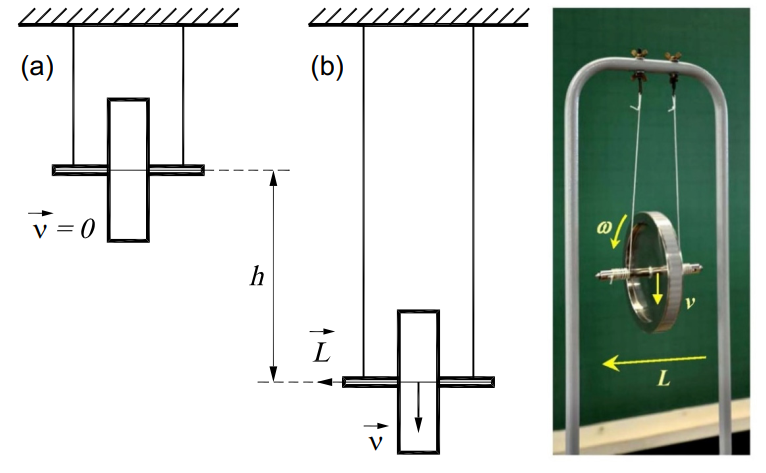
\includegraphics[scale=0.5]{images/setup-maxwell.png}
  \caption{Montagem experimental do Disco de Maxwell}
\end{figure}

Num primeiro momento, explodiremos o disco e utilizaremos as medidas de cara componente dele para determinar o seu momento de inércia, que será a soma dos momentos de cada componente. Como ele é feito de basicamente um cilindro inteiro (eixo) e 2 cilindros com furo (anel externo + disco), nós sabemos que o momento de inércia total será a soma dos momentos de inércia de cada peça:

\[I_T = I_E + I_A + I_D\]

E cada um desses componentes pode ser calculado a partir dessas 2 fórmulas para cilindros inteiros e cilindros com furo:

\[I_{CI} = \frac{1}{2}MR^2\]
\[I_{CF} = \frac{1}{2}M(R^2 + R_1^2)\]

Agora, vamos calcular por meio da queda o momento de inércia do disco. Para isso, primeiro precisaremos determinar uma altura \textit{h} para ser o nosso referencial de energia potencial gravitacional. Podemos utilizar o fio totalmente estendido como o ponto mais baixo, e a partir daí enrolar da forma que desejar. Após escolher tal altura será feito 3 medições do tempo de queda de acordo com o esquema (a) e (b) da figura anterior. Essas medições serão feitas com um cronometro de precisão.\\

Com 3 valores para \textit{$t_b$} - tempo para chegar no estado (b) - encontrados, podemos calcular o valor do momento de inércia \textit{I} do disco em estudo e utilizando a seguintes fórmula que foi deduzida na apostila do curso:

\[I = \left( \frac{gt_b^2}{2h} - 1 \right) mr^2\]

E a incerteza \textit{$\Delta$I} dessa medida será dada por:

\[\Delta I = \]

Após os cálculos podemos enfim fazer a comparação para ver se houve ou não conservação do momento de inércia, utilizando as seguintes desigualdades:

\[?\]

% =============== EXPERIMENTO 2 ===================== %

\subsection{Choques Rotacionais}

aaaaaaaaa

% =============== EXPERIMENTO 3 ===================== %

\subsection{Conservação do Momento Angular}

aaaaaaaa

% =============== EXPERIMENTO 4 ===================== %

\subsection{Precessão do Giroscópio}

O último experimento sobre esse tópico que vamos realizar é sobre giroscópios, mais precisamente o fenômeno da precessão que eles realizam, que consiste no movimento circular realizado em torno de um ponto de pivô por um objeto que gira, como pode ser visto nas figuras abaixo:

\begin{figure}[H]
  \centering
    \begin{subfigure}[b]{0.48\textwidth}
        \centering
        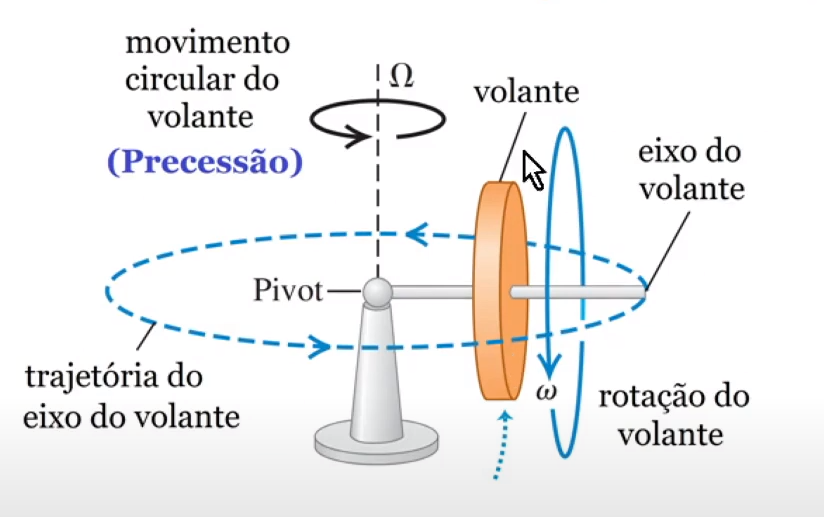
\includegraphics[width=\textwidth]{images/movimento-giroscopio.png}
        \caption{Diagrama do movimento de precessão de um giroscópio}
    \end{subfigure}
    \hfill
    \begin{subfigure}[b]{0.48\textwidth}
        \centering
        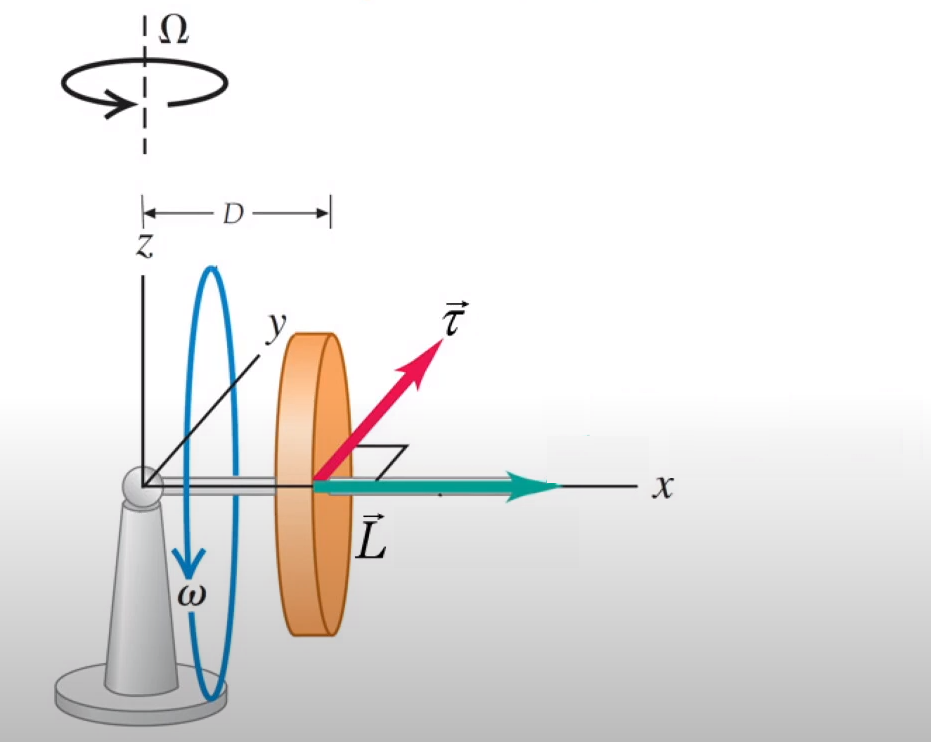
\includegraphics[width=\textwidth]{images/propriedades-giroscopio.png}
        \caption{Vetores que agem sobre o giroscópio}
    \end{subfigure}
\end{figure}

A partir dos diagramas acima, podemos realizar uma série de substituições de equações utilizando as equações básicas de rotação - como foi mostrado no vídeo dessa prática - para encontrar que a frequência da precessão $\Omega$ pode ser determinada pela seguinte equação:

\[ \Omega = \frac{MgD}{I \omega} \]

Com essa expressão em mãos podemos encontrar então o valor estimado da frequência de rotação do giroscópio $\Omega _e$.\\

Detalhe que para determinar \textit{I} haverá uma diferença nesse caso do giroscópio, pois diferente do Disco de Maxwell (tópico 2.1), não será possível desmontar a peça para pesar cada componente individualmente. Precisaremos calcular a massa da forma indireta, utilizando o valor da densidade do material que ela é feita.\\

Agora, como forma de comparação se soubermos o tempo que o giroscópio demora para fazer uma volta podemos calcular diretamente qual é a frequência de rotação $\Omega _d$ dada uma velocidade angular $\omega$ - que será medida utilizando um tacômetro. Esse valor $\Omega _d$ pode ser obtido pela simples relação:

\[ \Omega _d = \frac{2\pi}{\overline{t}} \]

% Onde $\overline{t}$ é o resultado da média aritmética dos
